\chapter{The Simulation Library}
\label{cha:the-simulation-library}

{\opp} has an extensive C++ class library which you can use when implementing
simple modules. Parts of the class library have already been covered in the
previous chapters:

\begin{itemize}
  \item{the message class \cclass{cMessage} (chapter \ref{cha:messages})}
  \item{sending and receiving messages, scheduling and canceling
    events, terminating the module or the simulation
    (section \ref{sec:simple-modules:sending-and-receiving})}
  \item{access to module gates and parameters via \cclass{cModule} member functions
    (sections \ref{sec:simple-modules:parameters} and \ref{sec:simple-modules:gates})}
  \item{accessing other modules in the network (section \ref{sec:simple-modules:walking-module-hierarchy})}
  \item{dynamic module creation (section \ref{sec:simple-modules:dynamic-module-creation})}
\end{itemize}

This chapter discusses the rest of the simulation library:

\begin{itemize}
  \item{random number generation: \ffunc{normal()},
    \ffunc{exponential()}, etc.}
  \item{module parameters: \cclass{cPar} class}
  \item{storing data in containers: the \cclass{cArray} and \cclass{cQueue} classes}
  \item{routing support and discovery of network topology: \cclass{cTopology} class}
  \item{recording statistics into files: \cclass{cOutVector} class}
  \item{collecting simple statistics: \cclass{cStdDev} and \cclass{cWeightedStddev} classes}
  \item{distribution estimation: \cclass{cLongHistogram},
    \cclass{cDoubleHistogram}, \cclass{cVarHistogram}, \cclass{cPSquare},
    \cclass{cKSplit} classes}
  \item{making variables inspectable in the graphical user interface (Tkenv):
        the \fmac{WATCH()} macros}
  \item{sending debug output to and prompting for user input in the graphical
    user interface (Tkenv\index{Tkenv}): the \ttt{ev}\index{ev} object (\cclass{cEnvir} class)}
\end{itemize}





\section{Class Library Conventions}

\subsection{Base Class}
\label{sec:ch-sim-lib:cobject}


Classes in the {\opp} simulation library are derived from \cclass{cOwnedObject}.
Functionality and conventions that come from \cclass{cOwnedObject}:
\begin{itemize}
  \item{name attribute}
  \item{\ffunc{getClassName()} member and other member functions giving textual
    information about the object}
  \item{conventions for assignment, copying, duplicating the object}
  \item{ownership\index{ownership} control for containers derived from \cclass{cOwnedObject}}
  \item{support for traversing the object tree}
  \item{support for inspecting the object in graphical user interfaces (Tkenv)}
\end{itemize}


Classes inherit and redefine several \cclass{cOwnedObject} member functions;
in the following we'll discuss some of the practically important
ones.


\subsection{Setting and Getting Attributes}

Member functions that set and query object attributes follow
a naming convention: the setter member function begins with
\ttt{set}, and the getter begins with \ttt{get} (or in the case of
boolean attributes, with \ttt{is} or \ttt{has}, whichever is more
appropriate). For example, the \textit{length} attribute of the
\cclass{cPacket} class can be set and read like this:

\begin{cpp}
pk->setBitLength(1024);
length = pk->getBitLength();
\end{cpp}

\begin{note}
    {\opp} 3.x and earlier versions did not have the \ttt{get} verb
    in the name of getter methods. There are scripts to port old source
    code to {\opp} 4.0; these tools and the suggested porting produre
    are described in the \textit{Migration Guide}.
\end{note}

\subsection{getClassName()}
\label{sec:sim-lib:classname}


For each class, the \ffunc{getClassName()} member function returns the class
name as a string:

\begin{cpp}
const char *className = msg->getClassName(); // returns "cMessage"
\end{cpp}


\subsection{Object Names}
\label{sec:sim-lib:name}

Gates, parameters and modules all have names in the NED files. At runtime,
those names are stored in the corresponding C++ objects, and are available 
for the code with the \ffunc{getName()} method. Other objects such as messages,
queues, result collection objects, etc. may also have names. 
  \footnote{Object name is inherited from \cclass{cObject} (which defines 
  \ffunc{getName()}), and from its subclass \cclass{cNamedObject} (which
  defines \ffunc{setName()} and actually stores the name string).}
Object names are generally very useful when you are tracing, debugging or 
demonstrating a simulation model.

For example, you can get the name of a message object like this:

\begin{cpp}
const char *name = msg->getName();
\end{cpp}

The \ffunc{getName()} method will never return \ttt{NULL}, the absence
of name string is always returned as the empty string (\ttt{""}).

By convention, the object name is the first argument to the constructor 
of every class, and it defaults to the empty string. To create an object with 
a name, pass the name string (a \ttt{const char *} pointer) as the first 
argument of the constructor:

\begin{cpp}
cMessage *timeoutMsg = new cMessage("timeout");
\end{cpp}

You can also change the name of an existing object:

\begin{cpp}
timeoutMsg->setName("timeout");
\end{cpp}

Both the constructor and \ffunc{setName()} make an internal copy of the string,
and not just store the pointer passed to them.
  \footnote{In a simulation, there are usually many objects with the same name:
  modules, parameters, gates, etc. To conserve memory, several classes
  keep names in a shared, reference-counted \textit{name pool} instead of
  making separate copies for each object. The runtime cost of looking up an 
  existing string in the name pool and incrementing its reference count 
  also compares favourably to the cost of allocation and copying.}

For convenience and efficiency reasons, the empty string \ttt{""}
and \ttt{NULL} are treated as interchangeable by library objects.
That is, \ttt{""} is stored as \ttt{NULL} but returned as \ttt{""}.
If you create a message object with either \ttt{NULL}
or \ttt{""} as name string, it will be stored as \ttt{NULL}
and \ffunc{getName()} will return a pointer to a static \ttt{""}.

\begin{cpp}
cMessage *msg = new cMessage(NULL, <additional args>);
const char *str = msg->getName(); // --> returns ""
\end{cpp}


\subsection{Object Full Name and Full Path}
\label{sec:sim-lib:fullname-and-fullpath}


Objects have two additional member functions that return strings
based on the object name: \ffunc{getFullName()} and \ffunc{getFullPath()}.
For gates and modules which are part of gate or module vectors,
\ffunc{getFullName()} returns the name with the index in brackets.
That is, for a module \ttt{node[3]} in the submodule vector \ttt{node[10]}
\ffunc{getName()} returns \ttt{"node"}, and \ffunc{getFullName()} returns \ttt{"node[3]"}.
For other objects, \ffunc{getFullName()} is the same as \ffunc{getName()}.

\ffunc{getFullPath()} returns \ffunc{getFullName()}, prepended with the
parent or owner object's \ffunc{getFullPath()} and separated by a dot.
That is, if the \ttt{node[3]} module above is in the compound module
\ttt{"net.subnet1"}, its \ffunc{getFullPath()} method will return
\ttt{"net.subnet1.node[3]"}.

\begin{cpp}
ev << this->getName();     // --> "node"
ev << this->getFullName(); // --> "node[3]"
ev << this->getFullPath(); // --> "net.subnet1.node[3]"
\end{cpp}

\ffunc{getClassName()}, \ffunc{getFullName()} and \ffunc{getFullPath()}
are extensively used on the graphical runtime environment Tkenv,
and also appear in error messages.

\ffunc{getName()} and \ffunc{getFullName()} return \ttt{const char *} pointers,
and \ffunc{getFullPath()} returns \ttt{std::string}. This makes no difference
with \ttt{ev<<}, but when \ffunc{getFullPath()} is used as a \ttt{"\%s"} argument
to \ffunc{sprintf()} you have to write \ttt{getFullPath().c\_str()}.

\begin{cpp}
char buf[100];
sprintf("msg is '%80s'", msg->getFullPath().c_str()); // note c_str()
\end{cpp}


\subsection{Copying and Duplicating Objects}


The \ffunc{dup()} member function creates an exact copy of the
object\index{object!copy}, duplicating\index{object!duplication}
contained objects also if necessary. This is especially useful in the
case of message objects.

\begin{cpp}
cMessage *copy = msg->dup();
\end{cpp}

\ffunc{dup()} delegates to the copy constructor, which in
turn relies on the assignment operator between objects.
\ffunc{operator=()} can be used to copy contents of an object into
another object of the same type. This is a deep copy: object
contained in the object will also be duplicated if necessary.
\ffunc{operator=()} does not copy the name string -- this task is done
by the copy constructor\index{copy constructor}.

\begin{note}
    Since the {\opp} 4.0 version, \ffunc{dup()} returns a pointer to
    the same type as the object itself, and not a \ttt{cObject*}.
    This is made possible by a relatively new C++ feature called
    \textit{covariant return types}.
\end{note}

\subsection{Iterators}


There are several container classes in the library (\cclass{cQueue},
\cclass{cArray} etc.) For many of them, there is a corresponding
iterator class that you can use to loop through the objects stored in
the container.

For example:

\begin{cpp}
cQueue queue;

//..
for (cQueue::Iterator queueIter(queue); !queueIter.end(); queueIter++)
{
    cOwnedObject *containedObject = queueIter();
}
\end{cpp}



\subsection{Error Handling}


When library objects detect an error condition, they throw a C++ exception.
%% NOTE we don't want to expose the actual C++ exception type, because
%% then people would start writing try-catch statements that'd make everything messy.
This exception is then caught by the simulation environment which pops up
an error dialog or displays the error message.

At times it can be useful to be able stop the simulation at the place of the error
(just before the exception is thrown) and use a C++ debugger to look
at the stack trace and examine variables. Enabling the \ttt{debug-on-errors}
ini file entry lets you do that -- check it in section
\ref{sec:ch-config-sim:general-section}  .

If you detect an error condition in your code, you can stop the
simulation with an error message using the \ffunc{opp\_error()} function.
\ttt{opp\_error()}'s argument list works like \ttt{printf()}: the
first argument is a format string which can contain \ttt{"\%s"}, \ttt{"\%d"} etc,
filled in using subsequent arguments.

An example:

\begin{cpp}
if (msg->getControlInfo()==NULL)
    opp_error("message (%s)%s has no control info attached",
              msg->getClassName(), msg->getName());
\end{cpp}



\section{Logging from Modules}

The logging feature will be used extensively in the code examples,
we introduce it here.

The \ttt{ev}\index{ev} object represents the user interface of the
simulation.  You can send debugging output to \ttt{ev} with the C++-style
output operators:

\begin{cpp}
ev << "packet received, sequence number is " << seqNum << endl;
ev << "queue full, discarding packet\n";
\end{cpp}

An alternative solution is \ffunc{ev.printf()}:

\begin{cpp}
ev.printf("packet received, sequence number is %d\n", seqNum);
\end{cpp}

The exact way messages are displayed to the user depends on the user
interface. In the command-line user interface (Cmdenv\index{Cmdenv}),
it is simply dumped to the standard output. (This output can also be
disabled from \ffilename{omnetpp.ini} so that it doesn't slow down simulation
when it is not needed.) In Tkenv, the runtime GUI, you can open
a text output window for every module.
It is not recommended that you use \ffunc{printf()} or \ffunc{cout}
to print messages -- \ttt{ev} output can be controlled much better
from \ffilename{omnetpp.ini} and it is more convenient to view, using Tkenv.

One can save CPU cycles by making logging statements conditional
on whether the output actually gets displayed or recorded anywhere.
The \ttt{ev.isDisabled()} call returns true when \ttt{ev<<} output is disabled,
such as in Tkenv or Cmdenv ``express'' mode. Thus, one can write code like
this:

\begin{cpp}
if (!ev.isDisabled())
    ev << "Packet " << msg->getName() << " received\n";
\end{cpp}

A more sophisticated implementation of the same idea is to the \fmac{EV}
macro which can be used in logging statements instead of \ttt{ev}.
One would simply write \ttt{EV<<} instead of \ttt{ev<<}:

\begin{cpp}
EV << "Packet " << msg->getName() << " received\n";
\end{cpp}

\ttt{EV}'s implementation makes use of the fact that the \ttt{<<} operator
binds looser than the conditional operator (\ttt{?:}).

%FIXME add tale about debug channels etc.


\section{Simulation Time Conversion}

Simulation time is represented by the type \ttt{simtime\_t}
which is a typedef to \ttt{double}.
{\opp} provides utility functions, which convert \ttt{simtime\_t}
to a printable string (\ttt{"3s 130ms 230us"}) and vica versa.

The \ffunc{simtimeToStr()} function converts a \cclass{simtime\_t}
(passed in the first argument) to textual form. The result is placed into
the \ttt{char} array pointed to by the second argument. If the second argument is omitted
or it is \ttt{NULL}, \ffunc{simtimeToStr()} will place the result into a
static buffer which is overwritten with each call. An example:

\begin{cpp}
char buf[32];
ev.printf("t1=%s, t2=%s\n", simtimeToStr(t1), simTimeToStr(t2,buf));
\end{cpp}

The \ffunc{simtimeToStrShort()} is similar to \ffunc{simtimeToStr()},
but its output is more concise.

The \ffunc{strToSimtime()} function parses a time specification passed
in a string, and returns a \cclass{simtime\_t}. If the string cannot
be entirely interpreted, -1 is returned.

\begin{cpp}
simtime_t t = strToSimtime("30s 152ms");
\end{cpp}

Another variant, \ffunc{strToSimtime0()} can be used if the time
string is a substring in a larger string. Instead of taking a \ttt{char*},
it takes a reference to \ttt{char*} (\ttt{char*\&}) as the first argument.  The
function sets the pointer to the first character that could not be
interpreted as part of the time string, and returns the value. It
never returns -1; if nothing at the beginning of the string looked
like simulation time, it returns 0.

\begin{cpp}
const char *s = "30s 152ms and something extra";

simtime_t t = strToSimtime0(s); // now s points to "and something extra"
\end{cpp}


\section{Generating Random Numbers}
\label{cha:sim-lib:generating-random-numbers}

Random numbers in simulation are never random. Rather, they are
produced using deterministic algorithms. Algorithms take a \textit{seed} value
and perform some deterministic calculations on them to produce
a ``random'' number and the next seed. Such algorithms and their
implementations are called \textit{random number generators} or RNGs,
or sometimes pseudo random number generators or PRNGs to highlight
their deterministic nature.
  \footnote{There are real random numbers as well, see e.g.
  http://www.random.org/, http://www.comscire.com, or the Linux
  \textit{/dev/random} device. For non-random numbers, try www.noentropy.net.}

Starting from the same seed, RNGs always produce the same sequence
of random numbers. This is a useful property and of great importance,
because it makes simulation runs repeatable.

RNGs produce uniformly distributed integers in some range,
usually between 0 or 1 and $2^{32}$ or so. Mathematical transformations
are used to produce random variates from them that correspond to
specific distributions.

\subsection{Random Number Generators}
\label{sec:sim-lib:rngs}
\index{random number generator}

\subsubsection{Mersenne Twister}

By default, {\opp} uses the Mersenne Twister RNG (MT) by M. Matsumoto and
T. Nishimura \cite{Matsumoto98}. MT has a period of $2^{19937}-1$,
and 623-dimensional equidistribution property is assured. MT is
also very fast: as fast or faster than ANSI C's \ttt{rand()}.

\subsubsection{The "Minimal Standard" RNG}

{\opp} releases prior to 3.0 used a linear congruential generator
(LCG) with a cycle length of $2^{31}-2$, described in
\cite{Jain91}, pp. 441-444,455. This RNG is still available
and can be selected from \ffilename{omnetpp.ini} (Chapter \ref{cha:run-sim}).
This RNG is only suitable for small-scale simulation studies.
As shown by Karl Entacher et al. in \cite{Entacher02},
the cycle length of about $2^{31}$ is too small (on todays
fast computers it is easy to exhaust all random numbers), and
the structure of the generated ``random'' points is too regular.
The \cite{Hellekalek98} paper provides a broader overview of issues
associated with RNGs used for simulation, and it is well worth reading.
It also contains useful links and references on the topic.

\subsubsection{The Akaroa RNG}

When you execute simulations under Akaroa control (see section
\ref{sec:ch-run-sim:akaroa}), you can also select Akaroa's
RNG as the RNG underlying for the {\opp} random number functions.
The Akaroa RNG also has to be selected from \ffilename{omnetpp.ini}
(section \ref{sec:ch-config-sim:rng-config}).

\subsubsection{Other RNGs}

{\opp} allows plugging in your own RNGs as well. This mechanism,
based on the \cclass{cRNG} interface, is described in section
\ref{sec:ch-plugin-exts:customization}.
For example, one candidate to include could be L'Ecuyer's CMRG \cite{LEcuyer02}
which has a period of about $2^{191}$ and can provide a large
number of \textit{guaranteed} independent streams.


\subsection{Random Number Streams, RNG Mapping}

Simulation programs may consume random numbers from several streams,
that is, from several independent RNG instances. For example, if a
network simulation uses random numbers for generating packets and
for simulating bit errors in the transmission, it might be a good
idea to use different random streams for both. Since the seeds
for each stream can be configured independently, this arrangement
would allow you to perform several simulation runs with the same traffic
but with bit errors occurring in different places.
A simulation technique called \textit{variance reduction} is
also related to the use of different random number streams.

It is also important that different streams and also different
simulation runs use non-overlapping series of random numbers.
Overlap in the generated random number sequences can introduce
unwanted correlation in your results.

The number of random number streams as well as seeds for the individual
streams can be configured in \ffilename{omnetpp.ini}
(section \ref{sec:ch-config-sim:rng-config}).
For the "minimal standard RNG", the \fprog{seedtool} program can be
used for selecting good seeds (section \ref{sec:ch-config-sim:seedtool}).

In {\opp}, streams are identified with RNG numbers. The RNG numbers
used in simple modules may be \textit{arbitrarily mapped} to the actual
random number streams (actual RNG instances) from \ffilename{omnetpp.ini}
(section \ref{sec:ch-config-sim:rng-config}). The mapping allows
for great flexibility in RNG usage and random number streams
configuration -- even for simulation models which were not written
with RNG awareness.


\subsection{Accessing The RNGs}

The \ffunc{intrand(n)} function generates random integers in the range $[0, n-1]$, and
\ffunc{dblrand()} generates a random double on $[0,1)$. These functions
simply wrap the underlying RNG objects. Examples:

\begin{cpp}
int dice = 1 + intrand(6); // result of intrand(6) is in the range 0..5
double p = dblrand();      // dblrand() produces numbers in [0,1)
\end{cpp}

They also have a counterparts that use generator \textit{k}:

\begin{cpp}
int dice = 1 + genk_intrand(k,6); // uses generator k
double prob = genk_dblrand(k);    // ""
\end{cpp}

The underlying RNG objects are subclassed from \cclass{cRNG},
and they can be accessed via \cclass{cModule}'s \ffunc{getRNG()} method.
The argument to \ffunc{getRNG()} is a local RNG number which will undergo
RNG mapping.

\begin{cpp}
cRNG *rng1 = getRNG(1);
\end{cpp}

\cclass{cRNG} contains the methods implementing the above \ffunc{intrand()}
and \ffunc{dblrand()} functions. The \cclass{cRNG} interface also allows
you to access the ``raw'' 32-bit random numbers generated by the RNG
and to learn their ranges (\ttt{intRand()}, \ttt{intRandMax()}) as well as
to query the number of random numbers generated (\ttt{getNumbersDrawn()}).


\subsection{Random Variates}

The following functions are based on \ffunc{dblrand()} and return
random variables of different distributions\index{distribution!random variables}\index{random!numbers from distributions}:

Random variate functions use one of the random number generators (RNGs)
provided by {\opp}. By default this is generator 0, but you can specify
which one to be used.

{\opp} has the following predefined distributions\index{distribution!predefined}:

\begin{longtable}{|p{6.5cm}|p{7.5cm}|}
\hline
\tbf{Function} & \tbf{Description}\\\hline
\multicolumn{2}{|c|}{\tbf{Continuous distributions}}\\\hline
\ffunc{uniform(a, b, \textit{rng=0})} & uniform distribution in the range [a,b) \\\hline
\ffunc{exponential(mean, \textit{rng=0})} & exponential distribution with the given mean \\\hline
\ffunc{normal(mean, stddev, \textit{rng=0})} & normal distribution with the given mean and standard deviation \\\hline
\ffunc{truncnormal(mean, stddev, \textit{rng=0})} & normal distribution truncated to nonnegative values \\\hline
\ffunc{gamma\_d(alpha, beta, \textit{rng=0})} & gamma distribution with parameters alpha>0, beta>0 \\\hline
\ffunc{beta(alpha1, alpha2, \textit{rng=0})} & beta distribution with parameters alpha1>0, alpha2>0 \\\hline
\ffunc{erlang\_k(k, mean, \textit{rng=0})} & Erlang distribution with k>0 phases and the given mean \\\hline
\ffunc{chi\_square(k, \textit{rng=0})} & chi-square distribution with k>0 degrees of freedom \\\hline
\ffunc{student\_t(i, \textit{rng=0})} & student-t distribution with i>0 degrees of freedom \\\hline
\ffunc{cauchy(a, b, \textit{rng=0})} & Cauchy distribution with parameters a,b where b>0 \\\hline
\ffunc{triang(a, b, c, \textit{rng=0})} & triangular distribution with parameters a<=b<=c, a!=c \\\hline
\ffunc{lognormal(m, s, rng=0)} & lognormal distribution with mean m and variance s>0 \\\hline
\ffunc{weibull(a, b, \textit{rng=0})} & Weibull distribution with parameters a>0, b>0 \\\hline
\ffunc{pareto\_shifted(a, b, c, \textit{rng=0})} & generalized Pareto distribution with parameters a, b and shift c \\\hline
\multicolumn{2}{|c|}{\tbf{Discrete distributions}} \\\hline
\ffunc{intuniform(a, b, \textit{rng=0})} & uniform integer from a..b \\\hline
\ffunc{bernoulli(p, \textit{rng=0})} & result of a Bernoulli trial with probability 0<=p<=1 (1 with probability p and 0 with probability (1-p)) \\\hline
\ffunc{binomial(n, p, \textit{rng=0})} & binomial distribution with parameters n>=0 and 0<=p<=1 \\\hline
\ffunc{geometric(p, \textit{rng=0})} & geometric distribution with parameter 0<=p<=1 \\\hline
\ffunc{negbinomial(n, p, \textit{rng=0})} & binomial distribution with parameters n>0 and 0<=p<=1\\\hline
\ffunc{poisson(lambda, \textit{rng=0})} & Poisson distribution with parameter lambda \\\hline

\end{longtable}


They are the same functions that can be used in NED files.
\ffunc{intuniform()} generates integers including both the lower and
upper limit, so for example the outcome of tossing a coin could be
written as intuniform(1,2).  \ffunc{truncnormal()} is the normal
distribution truncated to nonnegative values; its implementation
generates a number with normal distribution and if the result is
negative, it keeps generating other numbers until the outcome is
nonnegative.

If the above distributions don't suffice, you can write your own
functions\index{distribution!custom}. If you register your functions
with the \fmac{Register\_Function()} macro, you can use them in NED
files and ini files too.


\subsection{Random Numbers from Histograms}

You can also specify your distribution as a
histogram\index{distribution!as histogram}. The
\cclass{cLongHistogram}, \cclass{cDoubleHistogram},
\cclass{cVarHistogram}, \cclass{cKSplit} or \cclass{cPSquare} classes
are there to generate random numbers from equi\-dis\-tant-cell or
equiprobable-cell histograms.  This feature is documented later, with
the statistical classes.





\section{Container Classes}

\subsection{Queue class: cQueue}

\subsubsection{Basic Usage}


\cclass{cQueue} is a container class that acts as a queue.
\cclass{cQueue} can hold objects of type derived from \cclass{cOwnedObject}
(almost all classes from the {\opp} library), such as
\cclass{cMessage}, \cclass{cPar}, etc. Internally, \cclass{cQueue}
uses a double-linked list to store the elements.

A queue object has a head and a tail. Normally, new elements
are inserted at its head and elements are removed at its tail.


\begin{figure}[htbp]
  \begin{center}
    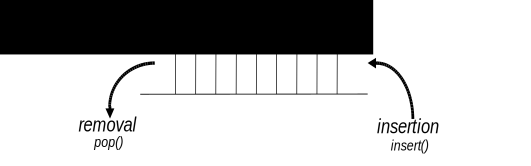
\includegraphics{figures/simlib-queue}
    \caption{cQueue: insertion and removal}
    \label{fig:ch-sim-lib:cqueue}
  \end{center}
\end{figure}

The basic \cclass{cQueue} member functions dealing with insertion and removal
are \ffunc{insert()} and \ffunc{pop()}. They are used
like this:

\begin{cpp}
cQueue queue("my-queue");
cMessage *msg;

// insert messages
for (int i=0; i<10; i++)
{
  msg = new cMessage;
  queue.insert(msg);
}

// remove messages
while(!queue.empty())
{
  msg = (cMessage *)queue.pop();
  delete msg;
}
\end{cpp}


The \ffunc{length()} member function returns the number of items in the
queue, and \ffunc{empty()} tells whether there is anything in the queue.

There are other functions dealing with insertion and removal.  The
\ffunc{insertBefore()} and \ffunc{insertAfter()} functions insert a
new item exactly before and after a specified one, regardless of the
ordering function.

The \ffunc{front()} and \ffunc{back()} functions return pointers to the objects
at the front and back of the queue, without affecting queue contents.

The \ffunc{pop()} function can be used to remove items from the
tail of the queue, and the \ffunc{remove()} function can be
used to remove any item known by its pointer from the queue:

\begin{cpp}
queue.remove(msg);
\end{cpp}



\subsubsection{Priority Queue}


By default, \cclass{cQueue} implements a FIFO, but it can also act as
a priority queue, that is, it can keep the inserted objects
ordered\index{queue!order}.  If you want to use this feature, you have
to provide a function that takes two \cclass{cOwnedObject} pointers,
compares the two objects and returns -1, 0 or 1 as the result (see the
reference for details).  An example of setting up an ordered
\cclass{cQueue}:

\begin{cpp}
cQueue sortedqueue("sortedqueue", cOwnedObject::cmpbyname, true );
                        // sorted by object name, ascending
\end{cpp}


If the queue object is set up as an ordered queue, the \ffunc{insert()}
function uses the ordering function: it searches the queue contents
from the head until it reaches the position where the new item
needs to be inserted, and inserts it there.


\subsubsection{Iterators}


Normally, you can only access the objects at the head or tail of the
queue. However, if you use an iterator class, \cclass{cQueue::Iterator},
you can examine each object in the queue\index{queue!iteration}.

The \cclass{cQueue::Iterator} constructor takes two arguments, the first
is the queue object and the second one specifies the initial position
of the iterator: 0=tail, 1=head. Otherwise it acts as any other
{\opp} iterator class: you can use the ++ and -- operators to advance
it, the () operator to get a pointer to the current item, and the
\ffunc{end()} member function to examine if you are at the end (or the
beginning) of the queue.


An example:

\begin{cpp}
for( cQueue::Iterator iter(queue,1); !iter.end(), iter++)
{
  cMessage *msg = (cMessage *) iter();
  //...
}
\end{cpp}




\subsection{Expandable Array: cArray}

\subsubsection{Basic Usage}


\cclass{cArray} is a container class that holds objects derived from
\cclass{cOwnedObject}. \cclass{cArray} stores the pointers of the objects
inserted instead of making copies. \cclass{cArray} works as an array,
but it grows automatically when it gets full. Internally,
\cclass{cArray} is implemented with an array of pointers; when the array
fills up, it is reallocated.

\cclass{cArray} objects are used in {\opp} to store parameters
attached to messages, and internally, for storing module parameters
and gates.


Creating an array:

\begin{cpp}
cArray array("array");
\end{cpp}

Adding an object at the first free index:

\begin{cpp}
cPar *p = new cMsgPar("par");
int index = array.add( p );
\end{cpp}


Adding an object at a given index (if the index is occupied,
you will get an error message):

\begin{cpp}
cPar *p = new cMsgPar("par");
int index = array.addAt(5,p);
\end{cpp}


Finding an object in the array:

\begin{cpp}
int index = array.find(p);
\end{cpp}

Getting a pointer to an object at a given index:

\begin{cpp}
cPar *p = (cPar *) array[index];
\end{cpp}

You can also search the array or get a pointer to an object by
the object's name:

\begin{cpp}
int index = array.find("par");
Par *p = (cPar *) array["par"];
\end{cpp}


You can remove an object from the array by calling \ffunc{remove()}
with the object name, the index position or the object pointer:

\begin{cpp}
array.remove("par");
array.remove(index);
array.remove( p );
\end{cpp}


The \ffunc{remove()} function doesn't deallocate the object, but it
returns the object pointer. If you also want to deallocate it, you can
write:

\begin{cpp}
delete array.remove( index );
\end{cpp}

\subsubsection{Iteration}


\cclass{cArray} has no iterator, but it is easy to loop through all the
indices with an integer variable. The \ffunc{size()} member function
returns the largest index plus one.

\begin{cpp}
for (int i=0; i<array.size(); i++)
{
  if (array[i]) // is this position used?
  {
    cOwnedObject *obj = array[i];
    ev << obj->getName() << endl;
  }
}
\end{cpp}


%
% \section{Non-object Container Classes}
%
% There are two container classes to store non-object
% items\index{non-object container}: \cclass{cLinkedList} and
% \cclass{cBag}.  The first one parallels with \cclass{cQueue}, the
% second one with \cclass{cArray}. They can be useful if you have to
% deal with C structs or objects that are not derived from
% \cclass{cOwnedObject}.
%
% See the class library reference for more info about them.
%


%FIXME document: cXMLElement
%FIXME document: simulation.getUniqueNumber(), for generating unique IDs for models


\section{Routing Support: cTopology}

\subsection{Overview}

The \cclass{cTopology} class was designed primarily to support
routing\index{routing support} in telecommunication or multiprocessor
networks.

A \cclass{cTopology} object stores an abstract representation of the
network in graph form:
\begin{itemize}
  \item{each \cclass{cTopology} node corresponds to a \textit{module}
    (simple or compound), and}
  \item{each \cclass{cTopology} edge corresponds to a \textit{link} or
    \textit{series of connecting links}.}
\end{itemize}

You can specify which modules (either simple or compound) you want to
include in the graph. The graph will include all connections among the
selected modules. In the graph, all nodes are at the same level,
there is no submodule nesting.  Connections which span across compound
module boundaries are also represented as one graph edge. Graph edges
are directed, just as module gates are.


If you are writing a router or switch model, the \cclass{cTopology}
graph can help you determine what nodes are available through which
gate and also to find optimal routes\index{optimal routes}. The
\cclass{cTopology} object can calculate shortest paths\index{shortest
  path} between nodes for you.

The mapping between the graph (nodes, edges) and network model
(modules, gates, connections) is preserved: you can easily find
the corresponding module for a \cclass{cTopology} node and vica versa.





\subsection{Basic Usage}

You can extract the network topology into a \cclass{cTopology}
object by a single function call. You have several ways to select
which modules you want to include in the topology:
\begin{itemize}
  \item{by module type}
  \item{by a parameter's presence and its value}
  \item{with a user-supplied boolean function}
\end{itemize}

First, you can specify which node types you want to include. The
following code extracts all modules of type \ttt{Router} or \ttt{Host}.
(\ttt{Router} and \ttt{Host} can be either simple or compound module types.)

\begin{cpp}
cTopology topo;
topo.extractByModuleType("Router", "Host", NULL);
\end{cpp}

Any number of module types can be supplied; the list must be terminated by \ttt{NULL}.

A dynamically assembled list of module types can be passed as a
\ttt{NULL}-terminated array of \ttt{const char*} pointers, or
in an STL string vector \ttt{std::vector<std::string>}.
An example for the former:

\begin{cpp}
cTopology topo;
const char *typeNames[3];
typeNames[0] = "Router";
typeNames[1] = "Host";
typeNames[2] = NULL;
topo.extractByModuleType(typeNames);
\end{cpp}

Second, you can extract all modules which have a certain parameter:

\begin{cpp}
topo.extractByParameter( "ipAddress" );
\end{cpp}

You can also specify that the parameter must have a certain value
for the module to be included in the graph:

\begin{cpp}
cMsgPar yes = "yes";
topo.extractByParameter( "includeInTopo", &yes );
\end{cpp}

The third form allows you to pass a function which can determine for
each module whether it should or should not be included.  You can have
\cclass{cTopology} pass supplemental data to the function through a
\ttt{void*} pointer. An example which selects all top-level modules (and
does not use the \ttt{void*} pointer):

\begin{cpp}
int selectFunction(cModule *mod, void *)
{
  return mod->getParentModule() == simulation.getSystemModule();
}

topo.extractFromNetwork( selectFunction, NULL );
\end{cpp}

%
% TBD one more example which \textit{does use} the void* ptr.
%

A \cclass{cTopology} object uses two types: \cclass{cTopology::Node} for
nodes and \cclass{cTopology::Link} for edges. (\cclass{sTopo\-Link\-In} and
\cclass{cTopology::LinkOut} are `aliases' for \cclass{cTopology::Link}; we'll
talk about them later.)

Once you have the topology extracted, you can start exploring
it. Consider the following code (we'll explain it shortly):

\begin{cpp}
for (int i=0; i<topo.getNumNodes(); i++)
{
  cTopology::Node *node = topo.getNode(i);
  ev << "Node i=" << i << " is " << node->getModule()->getFullPath() << endl;
  ev << " It has " << node->getNumOutLinks() << " conns to other nodes\n";
  ev << " and " << node->getNumInLinks() << " conns from other nodes\n";

  ev << " Connections to other modules are:\n";
  for (int j=0; j<node->getNumOutLinks(); j++)
  {
    cTopology::Node *neighbour = node->getLinkOut(j)->getRemoteNode();
    cGate *gate = node->getLinkOut(j)->getLocalGate();
    ev << " " << neighbour->getModule()->getFullPath()
       << " through gate " << gate->getFullName() << endl;
  }
}
\end{cpp}

The \ffunc{getNumNodes()} member function (1st line) returns the number of
nodes in the graph, and getNode(i) returns a pointer to the \textit{i}th
node, an \cclass{cTopology::Node} structure.


The correspondence between a graph node and a module can be obtained
by:

\begin{cpp}
cTopology::Node *node = topo.getNodeFor( module );
cModule *module = node->getModule();
\end{cpp}


The \ffunc{getNodeFor()} member function returns a pointer to the graph
node for a given module. (If the module is not in the graph, it
returns \ttt{NULL}). \ffunc{getNodeFor()} uses binary search within the
\cclass{cTopology} object so it is fast enough.


\cclass{cTopology::Node}'s other member functions let you determine the
connections of this node: \ffunc{getNumInLinks()}, \ffunc{getNumOutLinks()} return
the number of connections, \ttt{in(i)} and
\ttt{out(i)} return pointers to graph edge objects.


By calling member functions of the graph edge object, you can
determine the modules and gates involved. The \ffunc{getRemoteNode()}
function returns the other end of the connection, and
\ffunc{getLocalGate()}, \ffunc{getRemoteGate()}, \ffunc{getLocalGateId()} and
\ffunc{getRemoteGateId()} return the gate pointers and ids of the gates
involved. (Actually, the implementation is a bit tricky here: the same
graph edge object \cclass{cTopology::Link} is returned either as
\cclass{cTopology::LinkIn} or as \cclass{cTopology::LinkOut} so that ``remote''
and ``local'' can be correctly interpreted for edges of both
directions.)





\subsection{Shortest Paths}

The real power of \cclass{cTopology} is in finding shortest
paths\index{topology!shortest path} in the network to support optimal
routing\index{optimal routing}. \cclass{cTopology} finds shortest paths
from \textit{all} nodes \textit{to} a target node. The algorithm is
computationally inexpensive. In the simplest case, all edges are
assumed to have the same weight.

A real-life example when we have the target module pointer, finding
the shortest path looks like this:

\begin{cpp}
cModule *targetmodulep =...;
cTopology::Node *targetnode = topo.getNodeFor( targetmodulep );
topo.calculateUnweightedSingleShortestPathsTo( targetnode );
\end{cpp}


This performs the Dijkstra algorithm\index{Dijkstra algorithm} and
stores the result in the \cclass{cTopology} object. The result can
then be extracted using \cclass{cTopology} and
\ttt{cTopology::Node}\index{cTopology::Node} methods.  Naturally, each call to
\ffunc{calculateUnweightedSingleShortestPathsTo()} overwrites the results of
the previous call.

Walking along the path from our module to the target node:

\begin{cpp}
cTopology::Node *node = topo.getNodeFor( this );

if (node == NULL)
{
  ev < "We (" << getFullPath() << ") are not included in the topology.\n";
}
else if (node->getNumPaths()==0)
{
  ev << "No path to destination.\n";
}
else
{
  while (node != topo.getTargetNode())
  {
    ev << "We are in " << node->getModule()->getFullPath() << endl;
    ev << node->getDistanceToTarget() << " hops to go\n";
    ev << "There are " << node->getNumPaths()
       << " equally good directions, taking the first one\n";
    cTopology::LinkOut *path = node->getPath(0);
    ev << "Taking gate " << path->getLocalGate()->getFullName()
       << " we arrive in " << path->getRemoteNode()->getModule()->getFullPath()
       << " on its gate " << path->getRemoteGate()->getFullName() << endl;
    node = path->getRemoteNode();
  }
}
\end{cpp}


The purpose of the \ffunc{getDistanceToTarget()} member function of a
node is self-explanatory. In the unweighted case, it returns the
number of hops. The \ffunc{getNumPaths()} member function returns the number
of edges which are part of a shortest path, and
\ffunc[path()]{path(i)} returns the \textit{i}th edge of them as
\cclass{cTopology::LinkOut}. If the shortest paths were created by the
\ffunc[SingleShortestPaths()]{...SingleShortestPaths()} function,
\ffunc{getNumPaths()} will always return 1 (or 0 if the target is not
reachable), that is, only one of the several possible shortest paths
are found.  The
\ffunc[MultiShortestPathsTo()]{...MultiShortestPathsTo()} functions
find all paths, at increased run-time cost. The \cclass{cTopology}'s
\ffunc{getTargetNode()} function returns the target node of the last
shortest path search.

You can enable/disable nodes or edges in the graph. This is done by
calling their \ffunc{enable()} or \ffunc{disable()} member functions.
Disabled nodes or edges are ignored by the shortest paths calculation
algorithm. The \ffunc{isEnabled()} member function returns the state of
a node or edge in the topology graph.

One usage of \ffunc{disable()} is when you want to determine in how many
hops the target node can be reached from our node \textit{through
a particular output gate}. To calculate this, you calculate the
shortest paths to the target \textit{from the neighbor node}, but
you must disable the current node to prevent the shortest paths
from going through it:

\begin{cpp}
cTopology::Node *thisnode = topo.getNodeFor( this );
thisnode->disable();
topo.calculateUnweightedSingleShortestPathsTo( targetnode );
thisnode->enable();

for (int j=0; j<thisnode->getNumOutLinks(); j++)
{
  cTopology::LinkOut *link = thisnode->getLinkOut(i);
  ev << "Through gate " << link->getLocalGate()->getFullName() << " : "
     << 1 + link->getRemoteNode()->getDistanceToTarget() << " hops" << endl;
}
\end{cpp}

In the future, other shortest path algorithms will also be implemented:

\begin{cpp}
unweightedMultiShortestPathsTo(cTopology::Node *target);
weightedSingleShortestPathsTo(cTopology::Node *target);
weightedMultiShortestPathsTo(cTopology::Node *target);
\end{cpp}






\section{Statistics and Distribution Estimation}
\label{sec:ch-sim-lib:statistics}

\subsection{cStatistic and Descendants}

There are several statistic and result collection classes:
\cclass{cStdDev}, \cclass{cWeightedStdDev}, \cclass{Long\-Histogram},
\cclass{cDoubleHistogram}, \cclass{cVarHistogram}, \cclass{cPSquare} and
\cclass{cKSplit}. They are all derived from the abstract base class
\cclass{cStatistic}.

\begin{itemize}
  \item{\cclass{cStdDev} keeps the count, mean, standard
    deviation, minimum and maximum value etc of the observations.}
  \item{\cclass{cWeightedStdDev} is similar to \cclass{cStdDev}, but
    accepts weighted observations. \cclass{cWeightedStdDev} can be used
    for example to calculate time average. It is the only weighted
    statistics class.}
  \item{\cclass{cLongHistogram} and \cclass{cDoubleHistogram} are
    descendants of \cclass{cStdDev} and also keep an approximation of
    the distribution of the observations using equidistant
    (equal-sized) cell histograms\index{histogram!equal-sized}.}
  \item{\cclass{cVarHistogram} implements a histogram where cells do not
    need to be the same size. You can manually add the cell (bin)
    boundaries, or alternatively, automatically have a partitioning
    created where each bin has the same number of observations (or as
    close to that as possible).}
  \item{\cclass{cPSquare} is a class that uses the $P^{2}$ algorithm
    described in \cite{JCh85}. The algorithm calculates quantiles without
    storing the observations; one can also think of it as a histogram
    with equiprobable cells\index{histogram!equiprobable-cells}.}
  \item{\cclass{cKSplit} uses a novel, experimental method, based on an
    adaptive histogram-like algorithm.}
\end{itemize}

\subsubsection{Basic Usage}

One can insert an observation into a statistic object with the
\ffunc{collect()} function or the \texttt{+=} operator (they are
equivalent).  \cclass{cStdDev} has the following methods for getting
statistics out of the object: \ffunc{getCount()}, \ffunc{getMin()},
\ffunc{getMax()}, \ffunc{getMean()}, \ffunc{getStddev()}, \ffunc{getVariance()},
\ffunc{getSum()}, \ffunc{getSqrSum()} with the obvious meanings. An example
usage for \cclass{cStdDev}:

\begin{cpp}
cStdDev stat("stat");

for (int i=0; i<10; i++)
  stat.collect( normal(0,1) );

long numSamples = stat.getCount();
double smallest = stat.getMin(),
       largest = stat.getMax();
double mean = stat.getMean(),
       standardDeviation = stat.getStddev(),
       variance = stat.getVariance();
\end{cpp}





\subsection{Distribution Estimation}

\subsubsection{Initialization and Usage}

% TBD this has to be rewritten at some point... maybe take over examples from Doxygen doc.

The distribution estimation\index{distribution!estimation} classes
(\cclass{cLongHistogram}, \cclass{cDoubleHistogram}, \cclass{cVarHistogram},
\cclass{cPSquare} and \cclass{cKSplit}) are derived from
\cclass{cDensityEstBase}. Distribution estimation classes (except for
\cclass{cPSquare}) assume that the observations are within a range.
You may specify the range explicitly (based on some a-priori info
about the distribution), or you may let the object collect the first
few observations and determine the range from them.

The following member functions exist for setting up the range
and to specify how many observations should be used for automatically
determining the range (these methods are part of \cclass{cDensityEstBase}):

\begin{cpp}
setRange(lower,upper);
setRangeAuto(numFirstvals, rangeExtFactor);
setRangeAutoLower(upper, numFirstvals, rangeExtFactor);
setRangeAutoUpper(lower, numFirstvals, rangeExtFactor);
\end{cpp}

\begin{cpp}
setNumFirstVals(numFirstvals);
\end{cpp}

The following example creates a histogram with 20 cells and automatic
range estimation\index{histogram!range estimation}:

\begin{cpp}
cDoubleHistogram histogram("histogram", 20);
histogram.setRangeAuto(100,1.5);
\end{cpp}


Here, 20 is the number of cells (not including the underflow/overflow
cells, see later), and 100 is the number of observations to be
collected before setting up the cells. 1.5 is the range extension
factor. It means that the actual range of the initial observations
will be expanded 1.5 times and this expanded range will be used to lay
out the cells. This method increases the chance that further
observations fall in one of the cells and not outside the histogram
range.

\begin{figure}[htbp]
  \begin{center}
    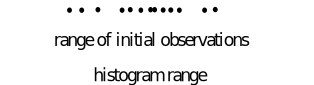
\includegraphics[width=3.215in, height=0.930in]{figures/simlib-histogramrange}
    \caption{Setting up a histogram's range}
  \end{center}
\end{figure}

The \ffunc{isTransformed()} function returns \textit{true} when the cells have
already been set up. You can force range estimation and setting
up the cells by calling the \ffunc{transform()} function.

The observations that fall outside the histogram range will be counted
as underflows and overflows. The number of underflows and overflows
are returned by the \ffunc{getUnderflowCell()} and \ffunc{getOverflowCell()}
member functions.

\begin{figure}[htbp]
\begin{center}
  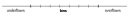
\includegraphics[width=3.310in, height=0.467in]{figures/simlib-histogramsetup}
  \caption{Histogram structure after setting up the cells}
\end{center}
\end{figure}

You create a $P^{2}$ object by specifying the number of cells:

\begin{cpp}
cPSquare psquare("interarrival-times", 20);
\end{cpp}

Afterwards, a \cclass{cPSquare} can be used with the same member functions
as a histogram.


\subsubsection{Getting Histogram Data}


There are three member functions to explicitly return cell boundaries
and the number of observations is each cell. \ffunc{getNumCells()} returns
the number of cells, \ffunc[getBasepoint()]{getBasepoint(int k)} returns the
\textit{k}th base point, \ffunc[getCellValue()]{getCellValue(int k)} returns the
number of observations in cell \textit{k}, and
\ffunc[getCellPDF()]{getCellPDF(int k)} returns the PDF value in the cell
(i.e. between \ffunc[getBasepoint()]{getBasepoint(k)} and
\ffunc[getBasepoint()]{getBasepoint(k+1)}).
The \ffunc[getCellInfo()]{getCellInfo(k)} method returns multiple data
(cell bounds, counter, relatile frequency) packed together in a struct.
These functions work for all histogram types, plus \cclass{cPSquare}
and \cclass{cKSplit}.

\begin{figure}[htbp]
  \begin{center}
    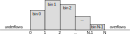
\includegraphics[width=2.615in, height=2.001in]{figures/simlib-histogramcells}
    \caption{base points and cells}
  \end{center}
\end{figure}

An example:

\begin{cpp}
long n = histogram.getCount();
for (int i=0; i<histogram.getNumCells(); i++)
{
  double cellWidth = histogram.getBasepoint(i+1)-histogram.getBasepoint(i);
  int count = histogram.getCellValue(i);
  double pdf = histogram.getCellPDF(i);
  //...
}
\end{cpp}


The \ffunc[getPDF()]{getPDF(x)} and \ffunc[getCDF()]{getCDF(x)} member functions
return the value of the Probability Density Function and the Cumulated
Density Function at a given \textit{x}, respectively.


\subsubsection{Random Number Generation from Distributions}


The \ffunc{random()} member function generates random
numbers\index{random!numbers} from the distribution stored by the
object:

\begin{cpp}
double rnd = histogram.random();
\end{cpp}


\cclass{cStdDev} assumes normal distribution.

The \cclass{cPar} object stores the pointer to the histogram (or $P^{2}$ object),
and whenever it is asked for the value, calls the histogram object's \ffunc{random()}
function:

\begin{cpp}
double rnd = (double)rndPar; // random number from the cPSquare
\end{cpp}

\subsubsection{Storing and Loading Distributions}


The statistic classes have \ffunc{loadFromFile()} member functions
that read the histogram data from a text file. If you need a custom
distribution\index{distribution!custom} that cannot be written (or it
is inefficient) as a C function, you can describe it in histogram form
stored in a text file, and use a histogram object with
\ffunc{loadFromFile()}.

You can also use \ffunc{saveToFile()}that writes out the distribution
collected by the histogram object:

\begin{cpp}
FILE *f = fopen("histogram.dat","w");
histogram.saveToFile(f); // save the distribution
fclose(f);

cDoubleHistogram hist2("Hist-from-file");
FILE *f2 = fopen("histogram.dat","r");
hist2.loadFromFile(f2); // load stored distribution
fclose(f2);
\end{cpp}


\subsubsection{Histogram with Custom Cells}


The \cclass{cVarHistogram} class can be used to create
histograms with arbitrary (non-equidistant) cells.
It can operate in two modes:

\begin{itemize}
  \item \textit{manual}, where you specify cell boundaries explicitly
     before starting collecting
  \item \textit{automatic}, where \ffunc{transform()} will set up the cells
     after collecting a certain number of initial observations. The cells
     will be set up so that as far as possible, an equal number of observations
     fall into each cell (equi-probable cells).
\end{itemize}

Modes are selected with a \textit{transform-type} parameter:
\begin{itemize}
  \item{\ttt{HIST\_TR\_NO\_TRANSFORM}: no transformation; uses bin boundaries
    previously defined by \ffunc{addBinBound()}}
  \item{\ttt{HIST\_TR\_AUTO\_EPC\_DBL}: automatically creates equiprobable cells}
  \item{\ttt{HIST\_TR\_AUTO\_EPC\_INT}: like the above, but for integers}
\end{itemize}

Creating an object:

\begin{cpp}
cVarHistogram(const char *s=NULL,
              int numcells=11,
              int transformtype=HIST_TR_AUTO_EPC_DBL);
\end{cpp}

Manually adding a cell boundary:

\begin{cpp}
void addBinBound(double x);
\end{cpp}

Rangemin and rangemax is chosen after collecting the
\texttt{numFirstVals} initial observations. One cannot add cell
boundaries when the histogram has already been transformed.





\subsection{The k-split Algorithm}

\subsubsection{Purpose}


The \textit{k}-split algorithm is an on-line distribution
estimation\index{distribution!online estimation} method.  It was
designed for on-line result collection in simulation programs.  The
method was proposed by Varga and Fakhamzadeh in 1997. The primary
advantage of \textit{k}-split is that without having to store the
observations, it gives a good estimate without requiring a-priori
information about the distribution, including the sample size. The
\textit{k}-split algorithm can be extended to multi-dimensional
distributions\index{distribution!multi-dimensional}, but here we deal
with the one-dimensional version only.


\subsubsection{The Algorithm}


The \textit{k-split} algorithm is an adaptive histogram-type estimate which
maintains a good partitioning by doing cell splits. We start out with
a histogram range $[x_{lo}, x_{hi})$ with $k$ equal-sized histogram
cells with observation counts $n_1,n_2, \cdots n_k$.  Each collected
observation increments the corresponding observation count. When an
observation count $n_i$ reaches a \textit{split threshold}, the cell
is split into $k$ smaller, equal-sized cells with observation counts
$n_{i,1}, n_{i,2}, \cdots n_{i,k}$ initialized to zero. The $n_i$
observation count is remembered and is called the \textit{mother
  observation count} to the newly created cells. Further observations
may cause cells to be split further (e.g. $n_{i,1,1},...n_{i,1,k}$
etc.), thus creating a $k$-order tree of observation counts where
leaves contain live counters that are actually incremented by new
observations, and intermediate nodes contain mother observation counts
for their children. If an observation falls outside the histogram
range, the range is extended in a natural manner by inserting new
level(s) at the top of the tree. The fundamental parameter to the
algorithm is the split factor $k$. Experience has shown that $k=2$
works best.

\begin{figure}[htbp]
  \begin{center}
    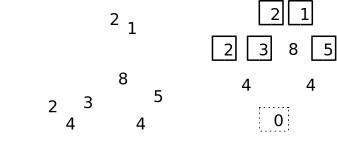
\includegraphics[width=3.442in, height=1.518in]{figures/simlib-ksplit1}
    \caption{Illustration of the k-split algorithm, $k=2$. The
      numbers in boxes represent the observation count values}
  \end{center}
\end{figure}


For density estimation, the total number of observations that
fell into each cell of the partition has to be determined. For
this purpose, mother observations in each internal node of the
tree must be distributed among its child cells and propagated
up to the leaves.

% careful with reformatting! $..$ MUST NOT BE BROKEN TO SEVERAL LINES!

Let $n_{...,i}$ be the (mother) observation count for a cell,
$s_{...,i}$ be the total observation count in a cell $n_{...,i}$ plus
the observation counts in all its sub-, sub-sub-, etc. cells), and
$m_{...,i}$ the mother observations propagated to the cell. We are
interested in the $\tilde{n}_{...,i} = n_{...,i} + m_{...,i}$
estimated amount of observations in the tree nodes, especially in the
leaves. In other words, if we have $\tilde{n}_{...,i}$ estimated
observation amount in a cell, how to divide it to obtain
$m_{...,i,1}, m_{...,i,2} \cdots m_{...,i,k}$
that can be propagated to child cells. Naturally,
$m_{...,i,1} + m_{...,i,2} + \cdots + m_{...,i,k} = \tilde{n}_{...,i}$.

% careful with reformatting! $..$ MUST NOT BE BROKEN TO SEVERAL LINES!

Two natural distribution methods are even
distribution\index{distribution!even} (when
$m_{...,i,1} = m_{...,i,2} = \cdots = m_{...,i,k}$) and proportional
distribution\index{distribution!proportional} (when
$m_{...,i,1} : m_{...,i,2} : \cdots : m_{...,i,k} = s_{...,i,1} : s_{...,i,2} : \cdots : s_{...,i,k}$).
Even distribution is optimal when the
$s_{...,i,j}$ values are very small, and proportional distribution is
good when the $s_{...,i,j}$ values are large compared to
$m_{...,i,j}$. In practice, a linear combination of them seems
appropriate, where $\lambda=0$ means even and $\lambda=1$ means
proportional distribution:

% careful with reformatting! $..$ MUST NOT BE BROKEN TO SEVERAL LINES!

$m_{\cdots,i,j} = (1-\lambda)\tilde{n}_{\cdots,i}/k + \lambda \tilde{n}_{\cdots,i} s_{...,i,j} / s_{\cdots,i}$
where $\lambda\in[0,1]$

\begin{figure}[htbp]
  \begin{center}
    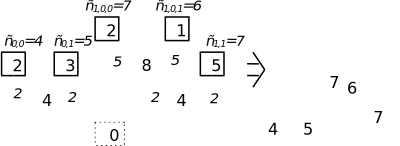
\includegraphics[width=4.147in, height=1.567in]{figures/simlib-ksplit2}
    \caption{Density estimation from the k-split cell tree. We
      assume $\lambda=0$, i.e. we distribute mother observations
      evenly.}
  \end{center}
\end{figure}

% careful with reformatting! $..$ MUST NOT BE BROKEN TO SEVERAL LINES!

Note that while $n_{...,i}$ are integers, $m_{...,i}$ and thus
$\tilde{n}_{...,i}$ are typically real numbers. The histogram estimate
calculated from \textit{k}-split is not exact, because the frequency
counts calculated in the above manner contain a degree of estimation
themselves. This introduces a certain \textit{cell division error};
the $\lambda$ parameter should be selected so that it minimizes that
error. It has been shown that the cell division error can
be reduced to a more-than-acceptable small value.\\
Strictly speaking, the \textit{k}-split algorithm is semi-online,
because its needs some observations to set up the initial histogram
range.  Because of the range extension and cell split
capabilities, the algorithm is not very sensitive to the choice of the
initial range, so very few observations are sufficient for range
estimation (say $N_{pre}=10$). Thus we can regard \textit{k}-split as
an on-line method.

\textit{K}-split can also be used in semi-online mode, when the
algorithm is only used to create an optimal partition from a larger
number of $N_{pre}$ observations. When the partition has been created,
the observation counts are cleared and the $N_{pre}$ observations are
fed into \textit{k}-split once again. This way all mother (non-leaf)
observation counts will be zero and the cell division error is
eliminated. It has been shown that the partition created by
\textit{k}-split can be better than both the equi-distant and the
equal-frequency partition.


{\opp} contains an implementation of the \textit{k}-split algorithm,
the \cclass{cKSplit} class.

\subsubsection{The cKSplit Class}

The \cclass{cKSplit} class is an implementation of the \textit{k-split} method.
Member functions:

%
% TBD comments
%

\begin{cpp}
void setCritFunc(KSplitCritFunc _critfunc, double *_critdata);
void setDivFunc(KSplitDivFunc \_divfunc, double *\_divdata);
void rangeExtension( bool enabled );
\end{cpp}


\begin{cpp}
int getTreeDepth();
int getTreeDepth(cKSplit::Grid& grid);
\end{cpp}

\begin{cpp}
double getRealCellValue(cKSplit::Grid& grid, int cell);
void printGrids();
\end{cpp}

\begin{cpp}
cKSplit::Grid& getGrid(int k);
cKSplit::Grid& getRootGrid();
\end{cpp}

\begin{cpp}
struct cKSplit::Grid
{
  int parent;   // index of parent grid
  int reldepth; // depth = (reldepth - rootgrid's reldepth)
  long total;   // sum of cells & all subgrids (includes "mother")
  int mother;   // observations "inherited" from mother cell
  int cells[K]; // cell values
};
\end{cpp}



\subsection{Transient Detection and Result Accuracy}

In many simulations, only the steady state performance (i.e.
the performance after the system has reached a stable state)
is of interest. The initial part of the simulation is called
the transient period. After the model has entered steady state,
simulation must proceed until enough statistical data has been
collected to compute result with the required accuracy.


Detection of the end of the transient period and a certain result
accuracy is supported by {\opp}. The user can attach transient
detection\index{transient detection} and result accuracy\index{result
  accuracy} objects to a result object (\cclass{cStatistic}'s
descendants). The transient detection and result accuracy objects will
do the specific algorithms on the data fed into the result object and
tell if the transient period is over or the result accuracy has been
reached.

The base classes for classes implementing specific transient
detection and result accuracy detection algorithms are:
\begin{itemize}
\item{\cclass{cTransientDetection}: base class for transient detection}
\item{\cclass{cAccuracyDetection}: base class for result accuracy detection}
\end{itemize}


\subsubsection{Basic Usage}

%
% TBD comments
%

Attaching detection objects to a \cclass{cStatistic} and getting pointers
to the attached objects:

\begin{cpp}
addTransientDetection(cTransientDetection *object);
addAccuracyDetection(cAccuracyDetection *object);
cTransientDetection *getTransientDetectionObject();
cAccuracyDetection *getAccuracyDetectionObject();
\end{cpp}


Detecting the end of the period:
\begin{itemize}
\item{polling the \ffunc{detect()} function of the object}
\item{installing a post-detect function}
\end{itemize}


\subsubsection{Transient Detection}


Currently one transient detection\index{transient detection} algorithm
is implemented, i.e.  there is one class derived from
\cclass{cTransientDetection}. The \cclass{cTDExpandingWindows} class
uses the sliding window approach with two windows, and checks the
difference of the two averages to see if the transient period is over.

\begin{cpp}
void setParameters(int reps=3,
                   int minw=4,
                   double wind=1.3,
                   double acc=0.3);
\end{cpp}

\subsubsection{Accuracy Detection}


Currently one accuracy detection\index{accuracy detection} algorithm
is implemented, i.e.  there is one class derived from
\cclass{cAccuracyDetection}. The algorithm implemented in the
\cclass{cADByStddev} class is: divide the standard deviation by the
square of the number of values and check if this is small enough.

\begin{cpp}
void setParameters(double acc=0.1, int reps=3);
\end{cpp}




\section{Recording Simulation Results}
\label{sec:ch-sim-lib:result-recording}

\subsection{Output Vectors: cOutVector}
\label{sec:ch-sim-lib:coutvector}

Objects of type \cclass{cOutVector} are responsible for writing time series
data (referred to as \textit{output vectors}) to a file. The \ffunc{record()}
method is used to output a value (or a value pair) with a timestamp.
The object name will serve as the name of the output vector.

The vector name can be passed in the constructor,

\begin{cpp}
cOutVector responseTimeVec("response time");
\end{cpp}

but in the usual arrangement you'd make the \cclass{cOutVector} a member
of the module class and set the name in \ffunc{initialize()}. You'd
record values from \ffunc{handleMessage()} or from a function called from
\ffunc{handleMessage()}.

The following example is a \ttt{Sink} module which records the lifetime
of every message that arrives to it.

\begin{cpp}
class Sink : public cSimpleModule
{
  protected:
    cOutVector endToEndDelayVec;

    virtual void initialize();
    virtual void handleMessage(cMessage *msg);
};

Define_Module(Sink);

void Sink::initialize()
{
    endToEndDelayVec.setName("End-to-End Delay");
}

void Sink::handleMessage(cMessage *msg)
{
    simtime_t eed = simTime() - msg->getCreationTime();
    endToEndDelayVec.record(eed);
    delete msg;
}
\end{cpp}

There is also a \ffunc{recordWithTimestamp()} method, to make it
possible to record values into output vectors with a timestamp other than
\ffunc{simTime()}. Increasing timestamp order is still enforced though.

All \cclass{cOutVector} objects write to a single \textit{output vector file}
that has a file extension \ttt{.vec}.
  \footnote{A \ttt{.vci} file is also created, but it is just an index for
  the \ttt{.vec} file and does not contain any new information. The IDE
  re-creates the \ttt{.vci} file if it gets lost.}
The format and processing of output vector files is described in section
\ref{cha:analyzing-simulation-results}.

You can configure output vectors from \ffilename{omnetpp.ini}:
you can disable individual vectors, or limit recording to certain
simulation time intervals (section \ref{sec:ana-sim:vector-config}).

If the output vector object is disabled or the simulation time is
outside the specified interval, \ffunc{record()} doesn't write
anything to the output file. However, if you have a Tkenv inspector
window open for the output vector object\index{output!vector object},
the values will be displayed there, regardless of the state of the
output vector object.



\subsection{Output Scalars}

While output vectors are to record time series data and thus they
typically record a large volume of data during a simulation run,
output scalars\index{output!scalars} are supposed to record a single
value per simulation run. You can use output scalars

\begin{itemize}
\item{to record summary data at the end of the simulation run}
\item{to do several runs with different parameter settings/random seed
    and determine the dependence of some measures on the parameter
    settings. For example, multiple runs and output scalars are the
    way to produce \textit{Throughput vs. Offered Load} plots.}
\end{itemize}

Output scalars are recorded with the \ffunc{record()} method of
\cclass{cSimpleModule}, and you will usually want to insert this code
into the \ffunc{finish()} function. An example:

\begin{cpp}
void Transmitter::finish()
{
    double avgThroughput = totalBits / simTime();
    recordScalar("Average throughput", avgThroughput);
}
\end{cpp}

You can record whole statistics objects by calling their \ffunc{record()}
methods, declared as part of \cclass{cStatistic}. In the following example
we create a \ttt{Sink} module which calculates the mean, standard
deviation, minimum and maximum values of a variable, and records them at the
end of the simulation.

\begin{cpp}
class Sink : public cSimpleModule
{
  protected:
    cStdDev eedStats;

    virtual void initialize();
    virtual void handleMessage(cMessage *msg);
    virtual void finish();
};

Define_Module(Sink);

void Sink::initialize()
{
    eedStats.setName("End-to-End Delay");
}

void Sink::handleMessage(cMessage *msg)
{
    simtime_t eed = simTime() - msg->getCreationTime();
    eedStats.collect(eed);
    delete msg;
}

void Sink::finish()
{
    recordScalar("Simulation duration", simTime());
    eedStats.record();
}
\end{cpp}

The above calls record the data into an \textit{output scalar file},
a line-oriented text file that has the file extension \ttt{.sca}.
The format and processing of output vector files is described in section
\ref{sec:ch-ana-sim:output-scalars}.



\section{Watches and Snapshots}

\subsection{Basic Watches}

It would be nice, but variables of type \ttt{int}, \ttt{long}, \ttt{double}
do not show up by default in Tkenv; neither do STL classes
(\ttt{std::string}, \ttt{std::vector}, etc.) or your own structs and
classes. This is because the simulation kernel, being a library, knows
nothing about types and variables in your source code.

{\opp} provides \fmac{WATCH()} and set of other macros to come to your rescue,
and make variable to be inspectable in Tkenv and to be output into the snapshot
file\index{snapshot file}. \fmac{WATCH()} macros are usually placed into
\ffunc{initialize()} (to watch instance variables) or to the top of the
\ffunc{activity()} function (to watch its local variables), the point being
that they should only be executed once.

\begin{cpp}
long packetsSent;
double idleTime;

WATCH(packetsSent);
WATCH(idleTime);
\end{cpp}

Of course, members of classes and structs can also be watched:

\begin{cpp}
WATCH(config.maxRetries);
\end{cpp}

When you open an inspector for the simple module in Tkenv and click
the Objects/Watches tab in it, you will see your watched variables
and their values there. Tkenv also lets you change the value of a
watched variable.

The \fmac{WATCH()} macro can be used with any type that has a
stream output operator (\ttt{operator<<}) defined. By default,
this includes all primitive types and \ttt{std::string}, but since
you can write \ttt{operator<<} for your classes/structs and basically
any type, \fmac{WATCH()} can be used with anything. The only limitation
is that since the output should more or less fit on single line, the
amount of information that can be conveniently displayed is limited.

An example stream output operator:

\begin{cpp}
std::ostream& operator<<(std::ostream& os, const ClientInfo& cli)
{
    os << "addr=" << cli.clientAddr << "  port=" << cli.clientPort; // no endl!
    return os;
}
\end{cpp}

And the \ttt{WATCH()} line:

\begin{cpp}
WATCH(currentClientInfo);
\end{cpp}


\subsection{Read-write Watches}

Watches for primitive types and \ttt{std::string} allow for changing
the value from the GUI as well, but for other types you need to explicitly
add support for that. What you need to do is define a stream input
operator (\ttt{operator>>}) and use the \fmac{WATCH\_RW()} macro instead of
\fmac{WATCH()}.

The stream input operator:

\begin{cpp}
std::ostream& operator>>(std::istream& is, ClientInfo& cli)
{
    // read a line from "is" and parse its contents into "cli"
    return is;
}
\end{cpp}

And the \ttt{WATCH\_RW()} line:

\begin{cpp}
WATCH_RW(currentClientInfo);
\end{cpp}


\subsection{Structured Watches}

\ttt{WATCH()} and \ttt{WATCH\_RW()} are basic watches: they allow one
line of (unstructured) text to be displayed. However, if you have a
data structure generated from message definitions (see Chapter \ref{cha:messages}),
then one can do better. The message compiler automatically generates
meta-information describing individual fields of the class or struct,
which makes it possible to display the contents on field level.

The \texttt{WATCH} macros to be used for this purpose are \fmac{WATCH\_OBJ()}
and \fmac{WATCH\_PTR()}. Both expect the object to be subclassed from
\cclass{cObject}; \fmac{WATCH\_OBJ()} expects a reference to such class,
and \fmac{WATCH\_PTR()} expects a pointer variable.

\begin{cpp}
ExtensionHeader hdr;
ExtensionHeader *hdrPtr;
...
WATCH_OBJ(hdr);
WATCH_PTR(hdrPtr);
\end{cpp}

CAUTION: With \fmac{WATCH\_PTR()}, the pointer variable must point to a valid
object or be \ttt{NULL} at all times, otherwise the GUI may crash
while trying to display the object. This practically means that
the pointer should be initialized to \ttt{NULL} even if not used, and
should be set to \ttt{NULL} when the object to which it points gets deleted.

\begin{cpp}
delete watchedPtr;
watchedPtr = NULL;  // set to NULL when object gets deleted
\end{cpp}


\subsection{STL Watches}

The standard C++ container classes (\ttt{vector}, \ttt{map}, \ttt{set}, etc)
also have structured watches, available via the following macros:

\fmac{WATCH\_VECTOR()}, \fmac{WATCH\_PTRVECTOR()},
\fmac{WATCH\_LIST()}, \fmac{WATCH\_PTRLIST()},
\fmac{WATCH\_SET()}, \fmac{WATCH\_PTRSET()},
\fmac{WATCH\_MAP()}, \fmac{WATCH\_PTRMAP()}.

The \ttt{PTR}-less versions expect the data items ("T") to have
stream output operators (\ttt{operator <<}), because that is how
they will display them. The \ttt{PTR} versions assume that
data items are pointers to some type which has \ttt{operator <<}.
\fmac{WATCH\_PTRMAP()} assumes that only the value type (``second'')
is a pointer, the key type (``first'') is not. (If you happen to use
pointers as key, then define \ttt{operator <<} for the pointer type
itself.)

Examples:

\begin{cpp}
std::vector<int> intvec;
WATCH_VECTOR(intvec);

std::map<std::string,Command*> commandMap;
WATCH_PTRMAP(commandMap);
\end{cpp}



\subsection{Snapshots}
\label{sec:ch-sim-lib:snapshots}

The \ffunc{snapshot()} function outputs textual information about all
or selected objects of the simulation (including the objects created
in module functions by the user) into the snapshot file\index{snapshot file}.

\begin{cpp}
bool snapshot(cOwnedObject *obj = &simulation, const char *label = NULL);
\end{cpp}

The function can be called from module functions, like this:

\begin{cpp}
snapshot();     // dump the whole network
snapshot(this); // dump this simple module and all its objects
snapshot(&simulation.msgQueue); // dump future events
\end{cpp}

This will append snapshot information to the end of the snapshot file.
(The snapshot file name has an extension of \ttt{.sna}, default is
\ttt{omnetpp.sna}\index{omnetpp.sna}. The actual file name can be set in the
config file.)

The snapshot file output is detailed enough to be used for debugging
the simulation: by regularly calling \ffunc{snapshot()}, one can trace
how the values of variables, objects changed over the simulation.
The arguments: label is a string that will appear in the output
file; obj is the object whose inside is of interest. By default,
the whole simulation (all modules etc) will be written out.

If you run the simulation with Tkenv, you can also create a snapshot
from the menu.

An example snapshot file (some abbreviations have been applied):

\begin{filelisting}
<?xml version="1.0" encoding="ISO-8859-1"?>
<snapshot object="simulation" label="Long queue" simtime="9.038229311343"
network="FifoNet">
  <object class="cSimulation" fullpath="simulation">
    <info></info>
    <object class="cCompoundModule" fullpath="FifoNet">
      <info>id=1</info>
      <object class="fifo::Source" fullpath="FifoNet.gen">
        <info>id=2</info>
        <object class="cPar" fullpath="FifoNet.gen.sendIaTime">
          <info>exponential(0.01s)</info>
          <detailedinfo>double sendIaTime = exponential(0.01s) @unit(s)
          </detailedinfo>
        </object>
        <object class="cGate" fullpath="FifoNet.gen.out">
          <info>--&gt; fifo.in</info>
        </object>
      </object>
      <object class="fifo::Fifo" fullpath="FifoNet.fifo">
        <info>id=3</info>
        <object class="cPar" fullpath="FifoNet.fifo.serviceTime">
          <info>0.01</info>
          <detailedinfo>double serviceTime = 0.01@unit(s)</detailedinfo>
        </object>
        <object class="cGate" fullpath="FifoNet.fifo.in">
          <info>&lt;-- gen.out</info>
        </object>
        <object class="cGate" fullpath="FifoNet.fifo.out">
          <info>--&gt; sink.in</info>
        </object>
        <object class="cQueue" fullpath="FifoNet.fifo.queue">
          <info>length=13</info>
          <object class="cMessage" fullpath="FifoNet.fifo.queue.job">
            <info>src=FifoNet.gen (id=2)  dest=FifoNet.fifo (id=3)</info>
          </object>
          <object class="cMessage" fullpath="FifoNet.fifo.queue.job">
            <info>src=FifoNet.gen (id=2)  dest=FifoNet.fifo (id=3)</info>
          </object>
        </object>
      <object class="fifo::Sink" fullpath="FifoNet.sink">
        <info>id=4</info>
        <object class="cGate" fullpath="FifoNet.sink.in">
          <info>&lt;-- fifo.out</info>
        </object>
      </object>
    </object>
    <object class="cMessageHeap" fullpath="simulation.scheduled-events">
      <info>length=3</info>
      <object class="cMessage" fullpath="simulation.scheduled-events.job">
        <info>src=FifoNet.fifo (id=3)  dest=FifoNet.sink (id=4)</info>
      </object>
      <object class="cMessage" fullpath="...sendMessageEvent">
        <info>at T=9.0464.., in dt=0.00817..; selfmsg for FifoNet.gen (id=2)</info>
      </object>
      <object class="cMessage" fullpath="...end-service">
        <info>at T=9.0482.., in dt=0.01; selfmsg for FifoNet.fifo (id=3)</info>
      </object>
    </object>
  </object>
</snapshot>

\end{filelisting}



% \subsection{Disabling Warnings}
%
% Some container classes and functions suspend the simulation and issue
% warning messages in potentially bogus/dangerous situations, for
% example when an object is not found and \ttt{NULL} pointer/reference is
% about to be returned. Very often this is useful, but sometimes it is
% more trouble. You can turn warnings on/off from the ini file
% (warnings=yes/no)\index{ini file!warnings}.
%
%
% It is a good practice to leave warnings\index{warnings} enabled, and
% temporarily disable warnings in places where {\opp} would normally
% issue warnings but you know the code is correct. This is done in the
% following way:
%
% \ begin{verbatim}
% bool w = simulation.warnings();
% simulation.setWarnings( false );
% ...
% ... // critical code
% ...
% simulation.setWarnings( w );
% \ end{verbatim}





\subsection{Getting Coroutine Stack Usage}

It is important to choose the correct stack size for
modules\index{module!stack size}\index{stack!size}.  If the stack is
too large, it unnecessarily consumes memory; if it is too small, stack
violation occurs.

From the Feb99 release, {\opp} contains a mechanism that detects stack
overflows\index{stack!overflow}. It checks the intactness of a
predefined byte pattern (\texttt{0xdeadbeef}) at the stack boundary,
and reports ``stack violation''\index{stack!violation} if it was
overwritten. The mechanism usually works fine, but occasionally it can
be fooled by large -- and not fully used -- local variables (e.g. char
buffer[256]): if the byte pattern happens to fall in the middle of
such a local variable, it may be preserved intact and {\opp} does not
detect the stack violation.

To be able to make a good guess about stack size, you can use
the \ffunc{getStackUsage()} call which tells you how much stack the module
actually uses. It is most conveniently called from \ffunc{finish()}:

\begin{cpp}
void FooModule::finish()
{
  ev << getStackUsage() <<  "bytes of stack used\n";
}
\end{cpp}


The value includes the extra stack added by the user interface library
(see \textit{extraStackforEnvir}\index{extraStackforEnvir} in
envir/omnetapp.h), which is currently 8K for Cmdenv and at least 16K
for Tkenv.
  \footnote{The actual value is platform-dependent.}

\ffunc{getStackUsage()}also works by checking the existence of predefined
byte patterns in the stack area, so it is also subject to the above
effect with local variables.



\section{Deriving New Classes}
\label{sec:ch-sim-lib:deriving-new-classes}

\subsection{cOwnedObject or Not?}

If you plan to implement a completely new class (as opposed to
subclassing something already present in {\opp}), you have
to ask yourself whether you want the new class to be based
on \cclass{cOwnedObject} or not.
Note that we are \textit{not} saying you should always
subclass from \cclass{cOwnedObject}.
Both solutions have advantages and disadvantages, which you
have to consider individually for each class.

\cclass{cOwnedObject} already carries (or provides a framework for)
significant functionality that is either relevant to
your particular purpose or not. Subclassing \cclass{cOwnedObject}
generally means you have more code to write (as you \textit{have to}
redefine certain virtual functions and adhere to conventions)
and your class will be a bit more heavy-weight.
However, if you need to store your objects in {\opp} objects like \cclass{cQueue}
or you'll want to store {\opp} classes in your object,
then you \textit{must} subclass from \cclass{cOwnedObject}.
  \footnote{For simplicity, in the these sections ``{\opp} object''
  should be understood as ``object of a class subclassed from
  \cclass{cOwnedObject}''}

The most significant features \cclass{cOwnedObject} has is
the name string (which has to be stored somewhere, so it has
its overhead) and ownership management (see section
\ref{sec:ch-sim-lib:ownership-management}) which
also has the advantages but also some costs.

As a general rule, small \ttt{struct}-like classes like \ttt{IPAddress},
\ttt{MACAddress}, \ttt{RoutingTableEntry}, \ttt{TCPConnectionDescriptor}, etc.
are better \textit{not} sublassed from \cclass{cOwnedObject}.
If your class has at least one virtual member function, consider
subclassing from \cclass{cObject}, which does not impose any
extra cost because it doesn't have data members at all, only
virtual functions.


\subsection{cOwnedObject Virtual Methods}

Most classes in the simulation class library are descendants of
\cclass{cOwnedObject}. If you want to derive a new class from
\cclass{cOwnedObject} or a \cclass{cOwnedObject} descendant, you must redefine
some member functions so that objects of the new type can fully
co-operate with other parts of the simulation system. A more or less
complete list of these functions is presented here. You don't need to
worry about the length of the list: most functions are not
absolutely necessary to implement. For example, you do not need to
redefine \ffunc{forEachChild()} unless your class is a container class.

The following methods \textbf{must} be implemented:

\begin{itemize}
  \item{\textit{Constructor}. At least two constructors should be provided:
        one that takes the object name string as \ttt{const char *}
        (recommended by convention), and another one with no arguments
        (must be present). The two are usually implemented as a single
        method, with \ttt{NULL} as default name string.}
  \item{\textit{Copy constructor}, which must have the following signature
        for a class \ttt{X}: \ttt{X(const X\&)}. The copy constructor is used
        whenever an object is duplicated. The usual implementation of
        the copy constructor is to initialize the base class with the
        name (\ffunc{getName()}) of the other object it receives, then call the
        assignment operator (see below).}
  \item{\textit{Destructor}.}
  \item{\textit{Duplication function,} \ffunc{X *dup() const}.
        It should create and return an exact duplicate of the object.
        It is usually a one-line function, implemented with the help
        of the \ttt{new} operator and the copy constructor.}
  \item{\textit{Assignment operator}, that is, \ttt{X\& operator=(const X\&)}
        for a class \ttt{X}. It should copy the contents of the other
        object into this one, except the name string. See later what to do
        if the object contains pointers to other objects.}
\end{itemize}

If your class contains other objects subclassed from \cclass{cOwnedObject},
either via pointers or as data member, the following function \textbf{should}
be implemented:

\begin{itemize}
  \item{\textit{Iteration function,} \ttt{void forEachChild(cVisitor *v)}.
        The implementation should call the function passed
        for each object it contains via pointer or as data member;
        see the API Reference on \cclass{cOwnedObject} on how to implement
        \ttt{forEachChild()}. \ffunc{forEachChild()} makes it possible
        for Tkenv to display the object tree to you, to perform searches on it, etc.
        It is also used by \ffunc{snapshot()} and some other library functions.}
\end{itemize}

The following methods are \textbf{recommended} to implement:

\begin{itemize}
  \item{\textit{Object info,} \ffunc{std::string info()}. The \ttt{info()} function
        should return a one-line string describing the object's contents or state.
        \ttt{info()} is displayed at several places in Tkenv.}
  \item{\textit{Detailed object info,} \ffunc{std::string detailedInfo()}.
        This method may potentially be implemented in addition to \ttt{info()};
        it can return a multi-line description. \ttt{detailedInfo()} is also
        displayed by Tkenv in the object's inspector.}
  \item{\textit{Serialization}, \ffunc{parsimPack()} and \ffunc{parsimUnpack()} methods.
        These methods are needed for parallel simulation, if you want
        objects of this type to be transmitted across partitions.}
\end{itemize}


\subsection{Class Registration}

You should also use the \fmac{Register\_Class()} macro to register the
new class. It is used by the \ffunc{createOne()} factory function, which can
create any object given the class name as a string. \ffunc{createOne()}
is used by the Envir library to implement \ffilename{omnetpp.ini} options
such as \ttt{rng-class="..."} or \ttt{scheduler-class="..."}.
(see Chapter \ref{cha:plugin-exts})

For example, an \ffilename{omnetpp.ini} entry such as

\begin{inifile}
rng-class = "cMersenneTwister"
\end{inifile}

would result in something like the following code to be executed
for creating the RNG objects:

\begin{cpp}
cRNG *rng = check_and_cast<cRNG*>(createOne("cMersenneTwister"));
\end{cpp}

But for that to work, we needed to have the following line somewhere in the code:

\begin{cpp}
Register_Class(cMersenneTwister);
\end{cpp}

\ffunc{createOne()} is also needed by the parallel distributed simulation feature
(Chapter \ref{cha:parallel-execution}) to create blank objects to unmarshal into
on the receiving side.


\subsection{Details}

We'll go through the details using an example. We create a new
class \ttt{NewClass}, redefine all above mentioned \cclass{cOwnedObject}
member functions, and explain the conventions, rules and tips
associated with them.
To demonstrate as much as possible, the class will contain
an \ttt{int} data member, dynamically allocated non-\cclass{cOwnedObject} data
(an array of \cclass{double}s),
an {\opp} object as data member (a \ttt{cQueue}), and
a dynamically allocated {\opp} object (a \ttt{cMessage}).

The class declaration is the following. It contains the declarations
of all methods discussed in the previous section.

\begin{cpp}
//
// file: NewClass.h
//
#include <omnetpp.h>

class NewClass : public cOwnedObject
{
  protected:
    int data;
    double *array;
    cQueue queue;
    cMessage *msg;
    ...
  public:
    NewClass(const char *name=NULL, int d=0);
    NewClass(const NewClass& other);
    virtual ~NewClass();
    virtual NewClass *dup() const;
    NewClass& operator=(const NewClass& other);

    virtual void forEachChild(cVisitor *v);
    virtual std::string info();
};
\end{cpp}

We'll discuss the implementation method by method.
Here is the top of the \ttt{.cc} file:

\begin{cpp}
//
// file: NewClass.cc
//
#include <stdio.h>
#include <string.h>
#include <iostream.h>
#include "newclass.h"

Register_Class( NewClass );


NewClass::NewClass(const char *name, int d) : cOwnedObject(name)
{
    data = d;
    array = new double[10];
    take(&queue);
    msg = NULL;
}
\end{cpp}

The constructor (above) calls the base class constructor with
the name of the object, then initializes its own data members.
You need to call \ffunc{take()} for \cclass{cOwnedObject}-based data members.


\begin{cpp}
NewClass::NewClass(const NewClass& other) : cOwnedObject(other.getName())
{
    array = new double[10];
    msg = NULL;
    take(&queue);
    operator=(other);
}
\end{cpp}

The copy constructor relies on the assignment operator. Because
by convention the assignment operator does not copy the
name member, it is passed here to the base class constructor.
(Alternatively, we could have written \ttt{setName(other.getName())}
into the function body.)

Note that pointer members have to be initialized (to \ttt{NULL} or to an
allocated object/memory) before calling the assignment operator,
to avoid crashes.

You need to call \ffunc{take()} for \cclass{cOwnedObject}-based data members.

\begin{cpp}
NewClass::~NewClass()
{
    delete [] array;
    if (msg->getOwner()==this)
        delete msg;
}
\end{cpp}

The destructor should delete all data structures the object allocated.
\cclass{cOwnedObject}-based objects should \textit{only} be deleted if they
are owned by the object -- details will be covered in section
\ref{sec:ch-sim-lib:ownership-management}.

\begin{cpp}
NewClass *NewClass::dup() const
{
    return new NewClass(*this);
}
\end{cpp}

The \ttt{dup()} functions is usually just one line, like the one above.

\begin{cpp}
NewClass& NewClass::operator=(const NewClass& other)
{
    if (&other==this)
        return *this;
    cOwnedObject::operator=(other);

    data = other.data;

    for (int i=0; i<10; i++)
        array[i] = other.array[i];

    queue = other.queue;
    queue.setName(other.queue.getName());

    if (msg && msg->getOwner()==this)
        delete msg;
    if (other.msg && other.msg->getOwner()==const_cast<cMessage*>(&other))
        take(msg = other.msg->dup());
    else
        msg = other.msg;
    return *this;
}
\end{cpp}

Complexity associated with copying and duplicating the object
is concentrated in the assignment operator, so it is usually
the one that requires the most work from you of all methods
required by \cclass{cOwnedObject}.

If you do not want to implement object copying and duplication,
you should implement the assignment operator to call
\ffunc{copyNotSupported()} -- it'll throw an exception that
stops the simulation with an error message if this function
is called.

The assignment operator copies contents of the \ttt{other} object
to this one, except the name string. It should always return
\ttt{*this}.

First, we should make sure we are not trying to copy the object
to itself, because it might be disastrous. If so (that is,
\ttt{\&other==this}), we return immediately without doing anything.

The base class part is copied via invoking the assignment operator of
the base class.

New data members are copied in the normal C++ way. If the class
contains pointers, you will most probably want to make a deep copy of
the data where they point, and not just copy the pointer values.

If the class contains pointers to {\opp} objects, you need
to take ownership into account. If the contained object is \textit{not owned}
then we assume it is a pointer to an ``external'' object, consequently
we only copy the pointer. If it is \textit{owned}, we duplicate
it and become the owner of the new object. Details of ownership
management will be covered in section \ref{sec:ch-sim-lib:ownership-management}.


\begin{cpp}
void NewClass::forEachChild(cVisitor *v)
{
    v->visit(queue);
    if (msg)
        v->visit(msg);
}
\end{cpp}

The \ffunc{forEachChild()} function should call \ttt{v->visit(obj)}
for each \ttt{obj} member of the class. See the API Reference for more
information of \ffunc{forEachChild()}.

\begin{cpp}
std::string NewClass::info()
{
    std::stringstream out;
    out << "data=" << data << ", array[0]=" << array[0];
    return out.str();

}
\end{cpp}

The \ffunc{info()} method should produce a concise, one-line string
about the object. You should try not to exceed 40-80 characters, since the
string will be shown in tooltips and listboxes.

See the virtual functions of \cclass{cObject} and \cclass{cOwnedObject}
in the class library reference for more information. The sources of the
Sim library (\ttt{include/}, \ttt{src/sim/}) can serve as further examples.



\section{Object Ownership Management}
\label{sec:ch-sim-lib:ownership-management}

\subsection{The Ownership Tree}

{\opp} has a built-in ownership management mechanism which
is used for sanity checks, and as part of the infrastructure
supporting Tkenv inspectors.

Container classes like \cclass{cQueue} own the objects inserted
into them. But this is not limited to objects inserted into a container:
\textit{every \cclass{cOwnedObject}-based object has an owner all the time}.
From the user's point of view, ownership is managed transparently.
For example, when you create a new \cclass{cMessage},
it will be owned by the simple module. When you send it, it will
first be handed over to (i.e. change ownership to) the FES\index{FES}, and,
upon arrival, to the destination simple module. When you encapsulate
the message in another one, the encapsulating message will become
the owner. When you decapsulate it again, the currently active
simple module becomes the owner.

The \ffunc{getOwner()} method, defined in \cclass{cOwnedObject}, returns the
owner of the object:

\begin{cpp}
cOwnedObject *o = msg->getOwner();
ev << "Owner of " << msg->getName() << " is: " <<
   << "(" << o->getClassName() << ") " << o->getFullPath() << endl;
\end{cpp}

The other direction, enumerating the objects owned can be implemented with
the \ffunc{forEachChild()} method by it looping through all
contained objects and checking the owner of each object.

\subsubsection{Why Do We Need This?}

The traditional concept of object ownership is associated with
the ``right to delete'' objects. In addition to that,
keeping track of the owner and the list of objects owned also
serves other purposes in {\opp}:

\begin{itemize}
    \item{enables methods like \ttt{getFullPath()} to be implemented.}

    \item{prevents certain types of programming errors, namely,
    those associated with wrong ownership handling.}

    \item{enables Tkenv to display the list of simulation objects
    present within a simple module. This is extremely useful for finding
    memory leaks caused by forgetting to delete messages that are
    no longer needed.}
\end{itemize}

Some examples of programming errors that can be caught
by the ownership facility:

\begin{itemize}
    \item{attempts to send a message while it is still in a queue,
    encapsulated in another message, etc.}

    \item{attempts to send/schedule a message while it is still owned
    by the simulation kernel (i.e. scheduled as a future event)}

    \item{attempts to send the very same message object to multiple
    destinations at the same time (ie. to all connected modules)}
\end{itemize}

For example, the \ffunc{send()} and \ffunc{scheduleAt()} functions check
that the message being sent/scheduled \textit{must} is owned by the module.
If it is not, then it signals a programming error: the message is probably
owned by another module (already sent earlier?), or currently scheduled, or
inside a queue, a message or some other object -- in either case, the
module does not have any authority over it. When you get the error message
(\ttt{"not owner of object"}), you need to carefully examine the error
message: which object has the ownership of the message, why's that, and
then probably you'll need to fix the logic somewhere in your program.

The above errors are easy to make in the code, and if not detected
automatically, they could cause random crashes which are usually very
difficult to track down. Of course, some errors of the same kind still
cannot be detected automatically, like calling member functions of a
message object which has been sent to (and so currently kept by) another
module.


\subsection{Managing Ownership}

Ownership is managed transparently for the user, but this mechanism
has to be supported by the participating classes themselves.
It will be useful to look inside \cclass{cQueue} and \cclass{cArray},
because they might give you a hint what behavior you need
to implement when you want to use non-{\opp} container classes
to store messages or other \cclass{cOwnedObject}-based objects.


\subsubsection{Insertion}

\cclass{cArray} and \cclass{cQueue} have internal data structures
(array and linked list) to store the objects which are inserted
into them. However, they do \textit{not} necessarily own all of these
objects.  (Whether they own an object or not can be determined
from that object's \ffunc{getOwner()} pointer.)

The default behaviour of \cclass{cQueue} and \cclass{cArray} is
to take ownership of the objects inserted.
This behavior can be changed via the \textit{takeOwnership} flag.

Here is what the \textit{insert} operation of \cclass{cQueue} (or \cclass{cArray}) does:
\begin{itemize}
    \item{insert the object into the internal array/list data structure}

    \item{if the \textit{takeOwnership} flag is true, take ownership
    of the object, otherwise just leave it with its original owner}
\end{itemize}

The corresponding source code:

\begin{cpp}
void cQueue::insert(cOwnedObject *obj)
{
    // insert into queue data structure
    ...

    // take ownership if needed
    if (getTakeOwnership())
        take(obj);

}
\end{cpp}


\subsubsection{Removal}

Here is what the \textit{remove} family of operations in \cclass{cQueue}
(or \cclass{cArray}) does:

\begin{itemize}
    \item{remove the object from the internal array/list data structure}

    \item{if the object is actually owned by this \cclass{cQueue}/\cclass{cArray},
    release ownership of the object, otherwise just leave it with
    its current owner}
\end{itemize}

After the object was removed from a \cclass{cQueue}/\cclass{cArray},
you may further use it, or if it is not needed any more, you can delete it.

The \textit{release ownership} phrase requires further explanation.
When you remove an object from a queue or array, the ownership
is expected to be transferred to the simple module's local objects list.
This is accomplished by the \ffunc{drop()} function, which transfers the
ownership to the object's default owner.
\ffunc{getDefaultOwner()} is a virtual method returning \ttt{cOwnedObject*}
defined in \cclass{cOwnedObject}, and its implementation returns
the currently executing simple module's local object list.

As an example, the \ffunc{remove()} method of \cclass{cQueue} is
implemented like this:
  \footnote{Actual code in \texttt{src/sim} is structured somewhat
  differently, but the meaning is the same.}

\begin{cpp}
cOwnedObject *cQueue::remove(cOwnedObject *obj)
{
    // remove object from queue data structure
    ...

    // release ownership if needed
    if (obj->getOwner()==this)
        drop(obj);

    return obj;
}
\end{cpp}


\subsubsection{Destructor}

The concept of \ffunc{ownership} is that \textit{the owner has the
exclusive right and duty to delete the objects it owns}.
For example, if you delete a \cclass{cQueue} containing \cclass{cMessage}s,
all messages it contains \textit{and} owns will also be deleted.

The destructor should delete all data structures the object allocated.
From the contained objects, only the owned ones are deleted -- that is,
where \ttt{obj->getOwner()==this}.


\subsubsection{Object Copying}

The ownership mechanism also has to be taken into consideration
when a \cclass{cArray} or \cclass{cQueue} object is duplicated.
The duplicate is supposed to have the same content as the
original, however the question is whether the contained objects
should also be duplicated or only their pointers taken over
to the duplicate \cclass{cArray} or \cclass{cQueue}.

The convention followed by \cclass{cArray}/\cclass{cQueue} is that
only owned objects are copied, and the contained but not owned ones
will have their pointers taken over and their original owners
left unchanged.

In fact, the same question arises in three places:
the assignment operator \ffunc{operator=()}, the copy constructor
and the \ffunc{dup()} method.
In {\opp}, the convention is that copying is implemented
in the assignment operator, and the other two just rely on it.
(The copy constructor just constructs an empty object and
invokes assignment, while \ffunc{dup()}
is implemented as \ffunc{new cArray(*this)}).

% FIXME finish this!
%
% \subsubsection{Another Example: cMessage's Encapsulation Feature}
%
% This template should be followed in other places too. Like cMessage's
% encapsulation...
%
% \ begin{verbatim}
% void cMessage::encapsulate(cMessage *msg)
% {
%     if (encapmsg)
%        throw cRuntimeException(this,"encapsulate(): another message already encapsulated");
%
%    if (msg)
%    {
%        if (msg->getOwner()!=&(simulation.getContextSimpleModule()->locals))
%            throw cRuntimeException(this,"encapsulate(): not owner of message");
%        take( encapmsg = msg );
%        len += encapmsg->len;
%    }
%}
%\ end{verbatim}
%
%
%\subsection{If you Use STL Containers}
%


%%% Local Variables:
%%% mode: latex
%%% TeX-master: "usman"
%%% End:
